\documentclass
	[ a4paper	% paper format
	, 12pt		% fontsize
	, twoside	% double-sided
	, openright	% begin new chapter on right side
	, notitlepage	% use no standard title page
	, parskip=half	% set paragraph skip to half of a line
	]{scrreprt}

\usepackage[english]{babel}
\usepackage{amsmath}
\usepackage{latexsym}
%\usepackage[mathletters]{ucs}
\usepackage{longtable}
\usepackage[T1]{fontenc}
\usepackage[utf8x]{inputenc}
\usepackage{graphicx}
\usepackage{tabularx}
\usepackage{color}			% Colors
\usepackage{colortbl}			% Table colors
\usepackage{makecell}			% Xhline
\usepackage{multirow}
\usepackage{caption}
%\usepackage{etoolbox}
\usepackage{amsfonts}
\usepackage{tikz}
\usepackage{fancyhdr}
\usepackage{amsthm}
\usepackage{amssymb}			% \blacklozenge
\usepackage{lscape}
\usepackage{hhline}
\usepackage{multicol}
\usepackage{lastpage}
\usepackage{mathtools}
\usepackage{tcolorbox}
\usepackage{minted}
\usepackage{csquotes}
\usepackage{geometry}
\usepackage[english]{babel}
\usepackage{fancyhdr}
\usepackage{parskip}
\usepackage{booktabs}
\usepackage[hidelinks]{hyperref}	% "hidelinks" removes the border around links

\geometry{
	a4paper,
	total	= {170mm, 257mm},
	left	= 20mm,
	top	= 30mm,
	bottom	= 30mm
}

\makeatletter
\AtBeginEnvironment{minted}{\dontdofcolorbox}
\def\dontdofcolorbox{\renewcommand\fcolorbox[4][]{##4}}
\makeatother

% Header and footer
% The use of "\chapter" forces "\pagestyle{plain}", therefore both page styles
% "plain" and "fancy" have to be set
\newcommand{\mystyle}{
	\fancyhf{}
	\lhead{Bern University of Applied Sciences}
	\rhead{Visualizing Geneva's Next Generation E-Voting System}
	\lfoot{}
	\cfoot{Page \thepage\ of \pageref{LastPage}}
	\rfoot{}
}

\pagestyle{fancy}
\mystyle
\fancypagestyle{plain}{\mystyle}

% Paragraph configuration
\setlength{\parindent}{1em}
\setlength{\parskip}{1em}

\usepackage{etoolbox}
\AtBeginEnvironment{minted}{\singlespacing%
    \fontsize{10}{10}\selectfont}

\newminted{python}{frame=lines,framerule=2pt}


\newcommand\tabularhead[1]{
\begin{table}[!hp]
  \caption{Use Case <<#1>>}
  \begin{tabular}{|p{0.3\linewidth}|p{0.7\linewidth}|}
    \hline
    \textbf{Use Case} & \textbf{#1} \\
    \hline}

  \newcommand\addrow[2]{#1 &#2\\ \hline}

  \newcommand\addmulrow[2]{ \begin{minipage}[t][][t]{2.5cm}#1\end{minipage}
     &\begin{minipage}[t][][t]{8cm}
      \begin{enumerate} #2   \end{enumerate}
      \end{minipage}\\ }

  \newenvironment{usecase}{\tabularhead}
{\hline\end{tabular}\end{table}}

\newcommand\tabularheadtestcase[1]{
\begin{table}[!hp]
  \caption{Test Case <<#1>>}
  \begin{tabular}{|p{0.2\linewidth}|p{0.8\linewidth}|}
    \hline
    \textbf{Test Case} & \textbf{#1} \\
    \hline}

  \newcommand\addstepsrow[2]{ \begin{minipage}[t][][t]{2.5cm}#1\end{minipage}
     &\begin{minipage}[t][][t]{11cm}
      \begin{enumerate} #2   \end{enumerate}
      \end{minipage}\\ }

  \newenvironment{testcase}{\tabularheadtestcase}
{\hline\end{tabular}\end{table}}


% Quotes
%\usepackage[autostyle, english = american]{csquotes}
%\MakeOuterQuote{"}

%\addto\captionsenglish{\def\figurename{Figure}}
%\addto\captionsenglish{\renewcommand{\chaptername}{Chapter}}
%\selectlanguage{english}

%\makeatletter
%\renewcommand{\@chapapp}{Chapter}
%\makeatother

%\tcbuselibrary{theorems}
%
%\theoremstyle{definition}
%\newtheorem{exmp}{Beispiel}[subsection]
%\renewcommand{\chaptername}{Chapter}
%\newmintinline['macro name']{'language'}{'options'}
%
%\newtcbtheorem[number within=section]{mytheo}{Theorem}
%{colback=green!5,colframe=green!35!black,fonttitle=\bfseries,before
%skip=20pt plus 2pt,after skip=20pt plus 2pt}{th}
%
%\makeatletter
%\def\@seccntformat#1{
%	\expandafter\ifx\csname c@#1\endcsname\c@subsection\else
%	\csname the#1\endcsname\quad
%	\fi
%}
%\makeatother


\begin{document}
%\pagestyle{empty} % hide header and footer on title page

\begin{titlepage}
\begin{center}
	\includegraphics[width=0.08\textwidth]{assets/bfh_logo.png}

	\vspace{1cm}

	\textsc{\LARGE Bern University of Applied Sciences (BFH)} \\[1.5cm]
	\textsc{\Large Bachelor Thesis} \\[0.5cm]

	\newcommand{\HRule}{\rule{\linewidth}{0.3mm}}
	\HRule \\[0.4cm]
	{\huge \bfseries CHVote Demonstrator} \\[0.3cm]
	\HRule \\[1.5cm]

	\begin{tabular}{rl}
	\textbf{Authored by}
	& Kevin \textsc{Häni} <\href{mailto:kevin.haeni@gmail.com}{kevin.haeni@gmail.com}> \\
	& Yannick \textsc{Denzer} <\href{mailto:yannick@denzer.ch}{yannick@denzer.ch}> \\
	\textbf{Supervised by}
	& Prof. Dr. Rolf \textsc{Haenni} <\href{mailto:rolf.haenni@bfh.ch}{rolf.haenni@bfh.ch}> \\
	\end{tabular}

	\vspace{1.5cm}


	\vfill

	Bern, {\large \today}
\end{center}
\end{titlepage}


\clearpage
\tableofcontents
%\listoftables
%\pagestyle{plain}

\clearpage
\chapter*{Management Summary}
The following documentation describes the context, planning and implementation of an application intended to visualize a new e-voting protocol. The protocol our application is based on is described in the paper "{}CHVote System Specification"{} of Rolf Haenni, Reto E. Koenig, Philipp Locher and Eric Dubuis of the Research Institute for Security in the Information Society (RISIS) of the Bern University of Applied Sciences. Their specifications describe how to build a next generation e-voting protocol which satisfies the complex requirements set up by the Swiss government, such as allowing an e-voting system to include large electorates.

Previous attempts to establish e-voting platforms in Switzerland were limited to only a small percentage of the electorate, for example Swiss citizens living abroad, because they only met the basic requirements, set up by the government. There exist many concepts and e-voting protocols which satisfy basic requirements, such as the privacy of the voters. However, an e-voting platform that could be used on a nationwide scale needs to be both individually and universally verifiable. This means in essence that an external individual can verify that all, but only valid votes have been counted in the tally. Current systems were behaving more like a black box and were not transparent enough to allow that kind of verification.

Another challenge which e-voting is facing is the educational problem: it is difficult to understand such a complex protocol without sufficient knowledge of cryptography. This might result in mistrust towards e-voting.

The goal of this project is to develop an application that addresses the educational problem of e-voting by allowing users to get a hands-on experience with the whole voting process from the perspective of each participating actor of the protocol. This would allow users to gain a better understanding of the next generation e-voting platform. The system should also be able to display multiple perspectives on different screens which requires real-time synchronization of data.

This document will first introduce the context of e-voting and our project task. Next it will describe the planning aspects such as the requirements and the time schedule. A short summary of the most important aspects of the CHVote protocol should establish the terminology and background knowledge for better understanding of our work. The main goal of this paper is to document in detail the implementation of our application, such as the architecture and the challenges we were facing. The document concludes with a short summary and reflection.

\chapter{Introduction}
\section{Electronic voting}
Since 2015, it is possible for Swiss citizens registered in the cantons Geneva and Neuchâtel and living abroad, to vote electronically. However, these systems did not yet meet the requirements in terms of security and transparency, to be accepted as a secure E-Voting platform on a nationwide scale.

One of the requirements that is hardest to achieve, is that a good e-voting system must be transparent and allow an external person to verify, that every protocol participant has abided by the protocol and that only valid votes have been counted. 

Another common problem is the \textbf{insecure platform problem}: If a voters computer is affected by malware, the vote casting process is no longer under the voters control and the candidate selection could be possibly manipulated without the voters notice. It must be \textbf{individually verifiable} to every voter that his intended vote has been received, while at the same time, the voters privacy must be ensured at all times. What sounds like a paradoxon, can be solved by modern cryptography.

A contract was formed between the state of Geneva and the Bern University of Applied Sciences to work out a new protocol which does meet the complex requirements set up by the government. In 2017, the resulting specification document has been officially published and a proof-of-concept / prototype has been successfully implemented by the State of Geneva. 

\section{The CHVote protocol}
The protocol our project is based on, does not originate from us! The concept and specification has been created by Rolf Haenni, Philipp Locher and Reto E. Koenig of the Institute for Security in the Information Society (RISIS) of the Bern University of Applied Sciences. For this project, we have implemented the protocol according to their specification. In this section we summarize the most important aspects of the protocol and establish the terminology for better understanding this document and our application.

\subsection{Actors}
A \textbf{voter} is a person who is eligible to vote in his respective state. Every voter must possess a voting card that has been sent to him prior to an election event and that contains several codes such as the voting code and the confirmation code, which are used to identify the voter during the vote casting process. Every voter is assigned a \textbf{counting circle} which typically corresponds to the voters municipal. This information is required for statistical purposes. 

A voter uses a \textbf{voting client} to participate in an election event, e.g. forming a ballot according to the protocol, by entering his selection, a voting code to cast, and later in the process, his confirmation code to confirm his vote. Verification codes and a finalization code are displayed by the voting client to ensure the voter that his vote has been cast as intended and hasn't been manipulated by a third party.

The \textbf{Election Administrator}, typically a person of the government, sets up the election event by providing the required information such as the candidates or the voters and initiates the generation of the cryptographic electorate data. He is also responsible for tallying the election and publishing the final results.

The \textbf{election authorities} can be seen as some kind of independent election observers. In a CHVote election event there are always multiple election authorities in order to avoid having a single authority that needs to be trusted. The authorities are involved in almost every step of the protocol, starting from generating their shares of the electorate data, shares of a jointly generated public key used for encryption, checking and responding to new ballots and vote confirmations, as well as in the mixing (a measure to ensure anonymity) and decryption phases.

The \textbf{Bulletin Board} acts as a central board over which most communication is done and where all the public data is stored.

The \textbf{Printing Authority} is responsible for printing the voting cards for all voters. Since the printing authority needs to be in possession of all the secret voting credentials, it is a very sensitive point in the protocol. The printed voting cards are handled over to a trusted mailing service for delivery.

\subsection{Pre-Election \& Voting cards}
Before the actual election phase, the vote administrator sets up the election event by entering all required parameters, namely the voters, the elections with their corresponding candidates and the number of candidates a voter can select in this respective election. All election authorities jointly generate the cryptographic data for the whole electorate from which the voting card information is derived. The printing authority combines the information from all election authorities, prints the voting cards and delivers them to the voters by a trusted mailing service. 

A voting card contains several codes, namely:

\begin{itemize}
	\item a voting code
	\item a confirmation code
	\item a finalization code
	\item one verification code for every candidate
\end{itemize}

The \textbf{voting and confirmation codes} are authentication codes and are used to authenticate the voter twice during the vote casting process; the first time with the voting code when he casts his vote, and a second time for confirming his vote. A second authentication code is required because otherwise an attacker who infected a voters computer with malware could just confirm a vote on behalf of the voter after he manipulated the candidate selection and skip the whole verification process w. 

\subsection{Individual verification with oblivious transfer}
As mentioned earlier, one of the big challenges of an evoting-protocol is how it deals with the insecure platform problem: A voting platform that is infected with malware poses the risk that an attacker can manipulate the candidate selection on the vote-casting page after the voter has entered his voting code. 

The CHVote specification suggests a "`Cast-as-intended verification"'-step to allow voters to detect this kind of manipulation: When a voter enters his voting code and the indices of his favored candidates, the voting client forms a \textbf{ballot} containing the voters selection encrypted with the authorities public key, his public voting credential derived from the voting code, and a \textbf{non-interactive zero knowledge proof} which proofs that the voter has formed the ballot according to the protocol and that he has been in knowledge of his voting code, without revealing any information about the voting code.

Every election authority has to check the voters public voting credential, the validity of the ballot proof and that the voter hasn't already cast a vote. The encrypted selection also serves as a query for an oblivious transfer. A \textbf{k-out-of-n oblivious transfer} allows a client to query a server for $k$ messages, without the server knowing what messages the client requested, and without the client learning anything about the other $n-k$ messages. Adapted to the CHVote protocol: The voting client queries the authorities for the corresponding verification codes of the selected candidates, without the authorities learning which candidates the voter has selected, and without revealing any information about the other candidates. 

The voter then checks if the returned verification codes match the codes of the candidates he has chosen on the printed voting card. If the selection was somehow manipulated by malware, the returned verification codes would not match the printed ones and the voter would have to abort the vote casting process. This way the integrity of the vote casting process can be guaranteed even in the presence of malware. In such a case, privacy on the other hand cannot be protected since the malware will learn the plaintext of the voters selection.

Another feature the protocol supports, is that an election event can consist of $t$ multiple parallel elections. In such cases, the voter has to submit a single ballot, which contains his candidate selection for all parallel elections. This raises the question, how the system can verify that a voter has chosen exactly the correct number of candidate in each election, and not for example one less in the first, and one additional candidate in the second election.

The specification suggests the following trick: Assuming an election consists of two parallel elections ($t=2$) with 3 candidates each ($n_1 = 3, n_2 = 3$), of which a voter can select one candidate in each election ($k_1 = k_2 =1$). The verification codes are derived from $n = \sum_{j=1}^{t} n_j$ random points on $t$ polynomials (one for every election event $j$) of degree $k_j - 1$, that each election authority has chosen randomly prior to the election. By learning exactly $k = \sum_{n=1}^{t} k_j$ points on these polynomials, the voting client is able to reproduce these polynomials and therefore is able to calculate a particular point with $x=0$ on these polynomials. The corresponding $y$ values are incorporated into the second credential from which the confirmation code is derived. As a result, only if a voter has been able to reconstruct these polynomials with the returned points by submitting a valid candidate selection, he will be able to confirm the vote that he casted.

\subsection{From homomorphic encryption to mix-networks}

Since there is still a connection between the encrypted ballot and the voter at this point, the encrypted selections are extracted from the ballots as the first step of the post-election phase. In order to anonymize the list of encryptions, every authority performs a cryptographic shuffle with a random permutation and re-encrypts all ciphertexts in order to make it impossible to find out which voter has submitted which encrypted ballot. This is done by using the multiplicative homomorphic property of the ElGamal encryption scheme. A multiplicative homomorphic encryption scheme allows to perform multiplications on the ciphertext such that:

\begin{equation*}Enc(a) \cdot Enc(b) = Enc(a \cdot b)\end{equation*}

The specification suggests multiplying the encryption with the encryption of the neutral element $1$ since this yields a new ciphertext for the exact same plaintext.

\subsection{Distributed trust}
The public key that is used for encrypting the ballots has been jointly generated by all election authorities. Therefore in order to decrypt the result, all authorities must provide their share of the private key. The measure of multiple authorities participating in the whole e-voting process ensures security of the whole election process as long as at least one election authority can be trusted.

\section{Project task}

Understanding such a complex protocol isn't easy and might be the reason why many people still do not trust electronic voting systems. In close consultation with the authors of the CHVote specification, we decided to develop an application that allows users to get a hands-on experience with the CHVote e-voting system and makes it possible to show and explain to an audience how the future of voting in Switzerland might possibly look like.

For this reason we have developed a web-based application which allows to visualize every step of a CHVote election event, from generating the electorate data, to casting and confirming ballots from a voters point of view, to the post-election processes like mixing, decryption and tallying. Opposed to a realistic prototype, the focus on our project is not to implement an e-voting-system that is totally realistic, but more on the visualization.  

As preparatory work, we have implemented all approximately 65 algorithms which were defined as pseudo-code in the CHVote specification document during the course "`Project 2"', which we have finished just before our bachelor thesis. From the resulting set of algorithms we have created a library which we used for implementing the protocol which our application will be built on.
%\chapter{CHVote Protocol}
\section{Protocol}
The protocol our solution is based on, does not originate from us! The concept and specification has been created by Rolf Haenni and his team at Institute for Security in the Information Society (RISIS) of the Bern University of Applied Sciences. For this project, we have implemented the protocol according to their specification. In this chapter we summarize the most important aspects of the protocol for better understanding our application.

\section{Goals}
As pointed out earlier, one of the big challenges an E-Voting protocol has to solve is the verifiability of the voting result while still ensuring the privacy of all voters. Another big problem e-voting systems are facing is the risk of a voting client being infected by malware which manipulates casting of a vote without the voters notice. Both of these issues are addressed by the use of modern cryptography.

\section{Protocol Participants}
\subsection{Voter}
A voter is a person who is eligible to vote in his state. Every voter must possess a voting card that has been sent to him prior to an election event and that contains several codes such as the voting code and the confirmation code, which are used to identify the voter during the vote casting process.

A voter uses a voting client (website) to form a ballot according to the protocol, by entering his selection, a voting code to cast, and later in the process, his confirmation code to confirm his vote. Verification codes and a finalization code are displayed by the voting client to ensure the voter that his vote has been cast as intended and hasn't been manipulated by a third party.
\subsection{Election Administrator}
The election administrator, typically a person of the government, sets up the election by providing the necessary information such as the candidates and the voters. He is also responsible for determining and publishing the final results of the election.
\subsection{Election Authorities}
The election authorities can be seen as some kind of observer. 
\subsection{Bulletin Board}
\subsection{Printing Authority}

\section{The basic idea of the CHVote protocol}
Before the actual election, voting sheets are generated and printed for the whole electorate and delivered to the voters by a trusted mailing service. The voting sheets contain several codes, namely:

\begin{itemize}
	\item voting code
	\item confirmation code
	\item finalization code
	\item one verification code for every candidate
\end{itemize}

The voting and confirmation code are authentication codes used to authenticate the voter.

The voter first selects candidates by entering their indices. The voting client then forms a ballot containing the voters selection encrypted with the authorities public key and authenticated with the voters personal voting code. Additionally, the ballot contains a query that queries the authorities for the corresponding verification codes of the selected candidates, without the server knowing which candidates the voter has selected. The voter then checks if the returned verification codes match the codes of the candidates he has chosen on the printed voting sheet. If the selection was somehow manipulated by malware, the returned verification codes would not match the printed ones and the voter would have to abort the vote casting process. This way the integrity of the vote casting can be assured even in the presence of malware. Privacy on the other hand cannot be protected since the malware will learn the plaintext of the voter's selection.

In order to verify that a voter has formed the ballot correctly by choosing exactly the number of candidates he is supposed to choose, the following trick is being used: the verification codes are derived from $n = \sum_{n=1}^{t} n_j$ random points on $t$ polynomials (one for every election event $j$) of degree $k_j - 1$, that each election authority has chosen randomly prior to the election. By learning exactly $k = \sum_{n=1}^{t} k_j$ points on these polynomials, the voting client is able to reproduce these polynomials and therefore is able to calculate a particular point with $x=0$ on these polynomials. The corresponding $y$ values are incorporated into the second voting credential from which the confirmation code is derived. Only if the voter knows these values (by submitting a valid candidate selection), he will be able to confirm the vote that he casted.

Since there is still a connection between the encrypted ballot and the voter at this point, the encrypted candidate selection is extracted from the ballots before tallying. After that, every authority is shuffling/mixing these encryptions in order to make it impossible to find out which voter has submitted which encrypted ballot. This mixing of the encrypted votes is done by using the homomorphic property of the ElGamal encryption scheme. Re-encryption of the ballots multiplied with the neutral element $1$ yields a new ciphertext for the same plaintext.

The public key that is used for encryption has been generated jointly by all authorities. Therefore in order to decrypt the result, all authorities must provide their share of the private key. The measure of multiple authorities participating in the whole e-voting process ensures the security of the whole election even if only one authority can be trusted.

\definecolor{vmcol}{RGB}{150,150,150}
\definecolor{nmcol}{RGB}{200,200,200}
\definecolor{zscol}{RGB}{83,142,213} % red: 217,151,149
\definecolor{zicol}{RGB}{194,214,154}

\newcommand{\zs}[0]{\cellcolor{zscol}}				% soll
\newcommand{\zi}[0]{\cellcolor{zicol}}				% ist
%\newcommand{\ms}[0]{\makebox[.613cm][r]{$\blacklozenge$}}	% Meilenstein
\newcommand{\ms}[1]{
	\makebox[.7cm][r]{
		\tikz[baseline=(char.base)]{
			\node[shape=circle,draw,inner sep=.02cm,fill=black,text=white] (char) { #1 };
		}
	}
}

\newcommand{\sq}[1]{\textcolor{#1}{\rule{.3cm}{.3cm}}}

\newcommand{\phase}[1]{
	\multicolumn{22}{l}{} \\
	\multicolumn{22}{l}{\cellcolor{gray!20}\textbf{#1}} \\ \hline
}

\chapter{Project Management}
This chapter describes the several aspects of the project planning such as the project method, the requirements and use-cases as well as the time schedule.

%\section{Project Method}%
Since this was not a project where the scope and goals were strictly defined and clear from the very beginning, it was important to elaborate the requirements in close collaboration with our supervisors early on. This is why we decided our project would be very suitable for an agile kind of project method. Because of the small team consisting of only two members, we did not choose a particular project method like SCRUM, as this would have probably caused more overhead than actual benefits.

We have therefore set up regular meetings (usually once every 2 weeks) with our supervisors to discuss our ideas and get feedback about the current progress.

\section{Goals}
As the first step, we have elaborated the goals and requirements for our application. We have structured the requirements into groups which correspond to the actors of the CHVote protocol and therefore the views our application is going to consist of.

Some requirements affect multiple or all actors and are therefore listed as "{}General Requirements"{}. We have also added a priority and requirement type to simplify the planning and time management.
\subsection{General Requirements}
\begin{longtable}{p{0.5cm}p{9cm}p{1cm}p{1cm}p{1cm}p{1cm}}
\hline
 & Description & Type & Prio. & Phase & Status\\
\hline
R1 & The CHVote protocol is implemented as specified in the latest specification document. The only exceptions are the algorithms for channel security. & Must & High & 1 & Done\\
R2 & The application is web-based and shows updates within the same demo-election event in real-time. & Must & High & 1 & Done\\
R3 & The system supports 1-out-of-3 type of elections (e.g. elect 1 of 3 possible candidates). & Must & High & 1 & Done\\
R4 & The system supports multiple parallel election events. & Must & High & 1 &  Done\\
R5 & Users can create new elections. & Must & High & 1 & Done \\
R6 & The system supports internationalization. Providing more than one language is not required. & Must & Med. & 1 & Done\\
R7 & The system can handle k-out-of-n type of elections. & Can & Med. & 1 & Done\\
\end{longtable}


\subsection{Election Overview}
\begin{longtable}{p{0.5cm}p{9cm}p{1cm}p{1cm}p{1cm}p{1cm}}
\hline
 & Description & Type & Prio. & Phase & Status\\
\hline
R8 & The overview shows which phase the election is currently in. & Must & High & 2 & Done\\
R9 & A graphical scheme of the CHVote protocol gives an overview of all participating parties. & Must & Med. & 2 & Done\\
\end{longtable}

\subsection{Election Administrator}
\begin{longtable}{p{0.5cm}p{9cm}p{1cm}p{1cm}p{1cm}p{1cm}}
\hline
 & Description & Type & Prio. & Phase & Status\\
\hline
R10 & An election can be set up by providing all required information such as the candidates, the number of parallel voters, the number of voters and the number of selections (simplified JSON input). & Must & High & 1 & Done\\
R11 & The election can be set up without entering the parameters in JSON format and allows an easier set up of elections with multiple parallel election events. & Must & Low & 2 & Done\\
R12 & The election administrator view allows to perform the tallying and displays the final result of an election in numbers and a pie chart. & Must & High & 1 & Done\\
R13 &  During election setup, the security parameters can be chosen from a set of predefined parameters. & Can & Low & 2 & Done\\
\end{longtable}

\subsection{Printing Authority}
\begin{longtable}{p{0.5cm}p{9cm}p{1cm}p{1cm}p{1cm}p{1cm}}
\hline
 & Description & Type & Prio. & Phase & Status\\
\hline
R14 & Users can generate and display voting cards for an election. & Must & High & 1 & Done\\
R15 & Voting cards hide sensitive information behind a scratch card. & Can & Med. & 2 & Done\\
\end{longtable}

\subsection{Election Authority}
\begin{longtable}{p{0.5cm}p{9cm}p{1cm}p{1cm}p{1cm}p{1cm}}
\hline
 & Description & Type & Prio. & Phase & Status\\
\hline
R16 & The election authority view shows all information known to the election authority. & Must & High & 1 & Done\\
R17 & After a voter has submitted a ballot, all election authorities can check and respond to the voter's submission. & Must & High & 1 & Done\\
R18 & In the post-election phase, all election authorities can perform the mixing and decryption tasks. & Must & High & 2 & Done\\
R19 & Each authority can optionally process all tasks automatically. & Can & High & 2 & Done\\
\end{longtable}


\subsection{Voter}
\begin{longtable}{p{0.5cm}p{9cm}p{1cm}p{1cm}p{1cm}p{1cm}}
\hline
 & Description & Type & Prio. & Phase & Status\\
\hline
R20 & Users are able to go through the whole vote-casting process for every voter. & Must & High & 1 & Done\\
R21 & The voting card of a voter is displayed on the screen. The voting and confirmation codes can be copied into the input textfields by double clicking. & Must & Med. & 1 & Done\\
\end{longtable}


\subsection{Bulletin Board}
\begin{longtable}{p{0.5cm}p{9cm}p{1cm}p{1cm}p{1cm}p{1cm}}
\hline
 & Description & Type & Prio. & Phase & Status\\
\hline
R22 & The bulletin board view shows which information is publicly available. & Must & High & 1 & Done\\
R23 & The bulletin board view is extended with verification functionality. & Can & Low & 2 & Done\\
\end{longtable}

\subsection{Out-of-Scope}
The following topics are considered out-of-scope for the duration of the project:
\begin{itemize}
	\item The goal of the project is not to build a realistic prototype. Therefore, the whole back-end will run on a single server while in a reality there would be components running on distributed servers. Another difference between our implementation and a productive implementation is that our application generates the ballots on the server. In a productive environment, the ballots would have to be generated on the client for security reasons. This, however, would require us to rewrite many of the already implemented algorithms in JavaScript.
	\item The protocol takes into account that not all voters might be eligible to vote in all elections of a given election event (eligibility matrix). For simplicity, we assume that all voters are eligible to vote in every election of our application.
	\item Message level encryption and signature based integrity protection are very important in a productive implementation of an e-voting system and are also described in the CHVote specifications. However, since our system is only used for demonstration purposes and we do not have a distributed infrastructure, there is no real need for channel security in the project.
	\item Providing more than one language is also out-of-scope. If there is enough time, a second language might be provided optionally.
\end{itemize}

\section{Time Schedule \& Implementation Phases}
As the next step, we created a time schedule and structured our project into smaller units of work.

The actual implementation phase has been broken down into two phases:

\begin{itemize}
	\item Phase 1 includes the implementation of all high priority must-requirements, which means basically developing an application that allows to visualize the whole CHVote election process. We have agreed that after phase 1 some parts of the user interface would still be in a rather primitive state (eg. user inputs and components used for data display will not yet be very user friendly and of more technical nature, for example in the JSON format).
	\item For phase 2 we planned implementing the can-requirements and all must-requirements with lower priority as well as improving the whole user experience.
\end{itemize}

This approach reduced the risk of hidden technical limitations of our architecture which could result in time-consuming architectural changes.

\begin{landscape}

\begin{table}[h]
\centering
\renewcommand{\arraystretch}{1.2}
\fontsize{2mm}{2mm}\selectfont
\begin{tabular}[c]{
	|m{7cm}|l
	*{10}{
		|>{\centering\arraybackslash}m{.3cm}
		|>{\centering\arraybackslash}m{.3cm}
	}
	|}

\hline

\textbf{Project Tasks} & & 38 & 39 & 40 & 41 & 42 & 43 & 44 & 45 & 46 & 47 & 48 & 49 & 50 & 51 & 52 & 53 & 54 \\ \hline

\phase{Documentation}
\multirow{2}{*}{Update documentation and journal}
& soll & \zs & \zs & \zs & \zs & \zs & \zs & \zs & \zs & \zs & \zs & \zs & \zs & \zs & \zs & \zs & \zs & \zs \ms{5} \\ \hhline{~*{21}{-}}
& ist  & \zi & \zi & \zi & & & \zi & & \zi & \zi & \zi & \zi & \zi & \zi & \zi & \zi &\zi & \zi \ms{5}\\ \hline

\phase{Concept}
\multirow{2}{*}{Working out goals / requirements}
& soll & \zs & \zs & \zs & & & & & & & & & & & & & & \\ \hhline{~*{21}{-}}
& ist  & \zi & \zi & \zi & \zi & \zi & & & & & & & & & & & & \\ \hline
\multirow{2}{*}{Concept}
& soll & & \zs & \zs & & & & & & & & & & & & & & \\ \hhline{~*{21}{-}}
& ist  & & \zi & \zi & \zi & & & & & & & & & & & & & \\ \hline

\phase{Implementation}
\multirow{2}{*}{Update CHVote cryptolibrary to the lastest specification}
& soll & \zs & \zs\ms{1} & & & & & & & & & & & & & & & \\ \hhline{~*{21}{-}}
& ist  & \zi & \zi\ms{1} & & & & & & & & & & & & & & & \\ \hline
\multirow{2}{*}{Prototyping (proof of concept)}
& soll & & & \zs & \zs\ms{2} & & & & & & & & & & & & & \\ \hhline{~*{21}{-}}
& ist  & & & \zi & \zi\ms{2} & & & & & & & & & & & & & \\ \hline

\phase{Iteration 1}
\multirow{2}{*}{Implement backend API}
& soll & & & & & \zs & \zs & \zs & \zs & \zs & \zs & & & & & & & \\ \hhline{~*{21}{-}}
& ist  & & & & & \zi & \zi & \zi & \zi & \zi & & & & & & & & \\ \hline
\multirow{2}{*}{Implement frontend: Pre-election}
& soll & & & & & & & \zs & \zs & & & & & & & & & \\ \hhline{~*{21}{-}}
& ist  & & & & & & & \zi & \zi & & & & & & & & & \\ \hline
\multirow{2}{*}{Implement frontend: Election}
& soll & & & & & & & & \zs & \zs & & & & & & & & \\ \hhline{~*{21}{-}}
& ist  & & & & & & & & \zi & \zi & & & & & & & & \\ \hline
\multirow{2}{*}{Implement frontend: Post-election}
& soll & & & & & & & & & \zs & \zs\ms{3} & & & & & & & \\ \hhline{~*{21}{-}}
& ist  & & & & & & & & & \zi & \zi\ms{3} & & & & & & & \\ \hline

\phase{Iteration 2}
\multirow{2}{*}{Automation of election authority (R19)}
& soll & & & & & & & & & & & \zs & & & & & & \\ \hhline{~*{21}{-}}
& ist  & & & & & & & & & & & \zi & & & & & & \\ \hline
\multirow{2}{*}{Voting Card layout, Scratchcard (R15)}
& soll & & & & & & & & & & & \zs & \zs & & & & & \\ \hhline{~*{21}{-}}
& ist  & & & & & & & & & & & \zi & \zi & & & & & \\ \hline
\multirow{2}{*}{Election Overview (R8, R9)}
& soll & & & & & & & & & & & & \zs & \zs & & & & \\ \hhline{~*{21}{-}}
& ist  & & & & & & & & & & & & & & & \zi & \zi & \zi \ms{4} \\ \hline
\multirow{2}{*}{k-out-of-n election types (R7)}
& soll & & & & & & & & & & & & & \zs & & & & \\ \hhline{~*{21}{-}}
& ist  & & & & & & & & & & & & & \zi & \zi & & & \\ \hline
\multirow{2}{*}{Improving the input forms and layout (R11)}
& soll & & & & & & & & & & & & & & \zs & & & \\ \hhline{~*{21}{-}}
& ist  & & & & & & & & & & & & & \zi & \zi & & & \\ \hline
\multirow{2}{*}{Flexible security level (R13)}
& soll & & & & & & & & & & & & & & & \zs & & \\ \hhline{~*{21}{-}}
& ist  & & & & & & & & & & & & & & \zi & & & \\ \hline
\multirow{2}{*}{Verifier functionality (R23) and reserve}
& soll & & & & & & & & & & & & & & & \zs & \zs\ms{4} &\\ \hhline{~*{21}{-}}
& ist  & & & & & & & & & & & & & & \zi & \zi & & \\ \hline
\phase{Project completion}
\multirow{2}{*}{Poster, Final Day, Presentation}
& soll & & & & & & & & & & & & & & & & \zs & \zs \\ \hhline{~*{21}{-}}
& ist  & & & & & & & & & & & & & & & & \zi &  \zi\\ \hline

\end{tabular}
\caption{Project schedule}
\end{table}

\end{landscape}

The following milestones have been defined based on the requirements:

\begin{itemize}
	\item M1: Implementation of the CHVote crypto-library is finished.
	\item M2: A proof-of-concept / prototype for our application has been drawn up.
	\item M3: Implementation phase 1 is finished (all must-criteria with a high priority are met).
	\item M4: Implementation phase 2 is finished (all requirements including the can-criteria are met).
	\item M5: The documentation is finished.
\end{itemize}

\section{Use Cases}
As the next step, we have converted the requirements into use cases, by grouping them according to the actors. One use case is shown as an example. Please refer to the appendix for a complete list of use cases.
\begin{usecase}{Casting of a vote}
	\addrow{Primary Actor}{Voter}
	\addrow{Description}{The voter can cast a vote by selecting his favored candidate(s) and his voting code}
	\addrow{Precondition}{
		\begin{itemize}
			\item The election has the status "{}Election Phase"{}
			\item A voter is selected in the voter view
			\item The voter has the status "{}Vote Casting Phase"{}
		\end{itemize}
	}
	\addrow{Postcondition}{The first election authority receives a ballot-check task}
	\addmulrow{Main path (M)}{
		\item The voter visits the voter view and selects his voter object
		\item The system demands a selection of the candidates and the voter's voting code
		\item The voter clicks on "{}Cast ballot"{}\\
	}
\end{usecase}

\chapter{CHVote Protocol}
Our project is based on the CHVote protocol specifications. We would like to point out, that this protocol and the followign ideas do not originate from us! The concept and specifications have been created by Rolf Haenni, Philipp Locher and Reto E. Koenig of the Institute for Security in the Information Society (RISIS) of the Bern University of Applied Sciences. For this project, we have implemented the protocol according to their specification. In this section we summarize the most important aspects of the protocol and establish the terminology for better understanding this document and our application

\section{Actors}
A \textbf{voter} is a person who is eligible to vote in his respective state. Every voter is assigned a \textbf{counting circle} which typically corresponds to the voters municipal and is required for statistical purposes. For authentication purposes, every voter must possess a voting card that has been sent to him prior to an election event that contains codes used to identify the voter during the vote casting process.

The \textbf{Election Administrator}, typically a person of the government, is responsible for setting up the election event by providing the required information such as the candidates or the voters and initiates the generation of the cryptographic electorate data. He is also responsible for tallying the election and publishing the final results.

The \textbf{election authorities} can be seen as some kind of independent election observers. In a CHVote election event there are always multiple election authorities in order to avoid having to trust a single authority. The authorities are involved in almost every step of the protocol, starting from the generation of their shares of the electorate data, checking and responding to new ballots, as well as in the mixing (a measure to ensure anonymity) and decryption phases. The public key that is used for encrypting the ballots has been jointly generated by all election authorities. Therefore in order to decrypt the ballots, all authorities must work together and provide their share of the private key. 

The measure of multiple authorities participating in the whole e-voting process establishes a \textbf{distribution of trust} and ensures security of the whole election process as long as at least one election authority can be trusted.

The \textbf{Bulletin Board} acts as a central board over which most communication is done and where all the public data is stored. By publishing all data that is not secret onto a public board, including the list of encrypted ballots, and functionality to verify the correctness of these data, the protocol is making a big step towards the demanded transparency and the universal verification.

The \textbf{Printing Authority} is responsible for printing the voting cards for all voters. Since the printing authority needs to be in possession of all the secret voting codes, it is a very sensitive point in the protocol. The printed voting cards are handled over to a trusted mailing service for delivery.

\section{Pre-Election \& Voting Cards}
Before the actual election phase, the vote administrator sets up the election event by entering all required parameters, including the voters, the elections with their corresponding candidates and the number of candidates a voter can select in every election. All election authorities jointly generate the cryptographic data for the whole electorate from which the voting card information is derived. The printing authority combines the information from all election authorities, prints the voting cards and delivers them to the voters by a trusted mailing service. 

A voting card contains several codes, namely:

\begin{itemize}
	\item a voting code
	\item a confirmation code
	\item a finalization code
	\item one verification code for every candidate
\end{itemize}

The \textbf{voting and confirmation codes} are authentication codes and are used to authenticate the voter twice during the vote casting process; the first time with the voting code when he casts his vote, and a second time for confirming his vote. A second authentication code is required because otherwise an attacker who infected a voters computer with malware could just confirm a vote on behalf of the voter after he manipulated the candidate selection and could therefore skip the whole verification process.

\section{Vote casting with oblivious transfers}
As mentioned earlier, one of the big challenges of an evoting-protocol is how it deals with the insecure platform problem: A voting platform that is infected with malware poses the risk that an attacker can manipulate the candidate selection on the vote-casting page after the voter has entered his voting code. 

The CHVote specification suggests a "`Cast-as-intended verification"'-step to allow voters to detect this kind of manipulation: When a voter enters his voting code and the indices of his favored candidates, the voting client forms a \textbf{ballot} containing the voters selection encrypted with the authorities public key, his public voting credential derived from the voting code, and a \textbf{non-interactive zero knowledge proof} which proofs that the voter has formed the ballot according to the protocol and that he has been in knowledge of his voting code, without revealing any information about the voting code.

Every election authority has to check the voters public voting credential, the validity of the ballot proof and that the voter hasn't already cast a vote. The encrypted selection also serves as a query for an oblivious transfer. A \textbf{k-out-of-n oblivious transfer} allows a client to query a server for $k$ messages, without the server knowing what messages the client requested, and without the client learning anything about the other $n-k$ messages. Adapted to the CHVote protocol: The voting client queries the authorities for the corresponding verification codes of the selected candidates, without the authorities learning which candidates the voter has selected, and without revealing any information about the other candidates. 

The voter then checks if the returned verification codes match the codes of the candidates he has chosen on the printed voting card. If the selection was somehow manipulated by malware, the returned verification codes would not match the printed ones and the voter would have to abort the vote casting process. This way the integrity of the vote casting process can be guaranteed even in the presence of malware. In such a case, privacy on the other hand cannot be protected since the malware will learn the plaintext of the voters selection.

Another feature the protocol supports, is that an election event can consist of $t$ multiple parallel elections. In such cases, the voter has to submit a single ballot, which contains his candidate selection for all parallel elections. This raises the question, how the system can verify that a voter has chosen exactly the correct number of candidate in each election, and not for example one less in the first, and one additional candidate in the second election.

The specification suggests the following trick: Assuming an election consists of two parallel elections ($t=2$) with 3 candidates each ($n_1 = 3, n_2 = 3$), of which a voter can select one candidate in each election ($k_1 = k_2 =1$). The verification codes are derived from $n = \sum_{j=1}^{t} n_j$ random points on $t$ polynomials (one for every election event $j$) of degree $k_j - 1$, that each election authority has chosen randomly prior to the election. By learning exactly $k = \sum_{n=1}^{t} k_j$ points on these polynomials, the voting client is able to reproduce these polynomials and therefore is able to calculate a particular point with $x=0$ on these polynomials. The corresponding $y$ values are incorporated into the second credential from which the confirmation code is derived. As a result, only if a voter has been able to reconstruct these polynomials with the returned points by submitting a valid candidate selection, he will be able to confirm the vote that he casted.

\section{Anonymity with a Рe-Еncryption Mix-Net}

As mentioned earliert, both the election authorities as well as the bulletin board keep track of all the casted ballots, which contains the voters candidate selection encrypted under the public key that has been jointly generated by all election authorities. Up to this point, the ballots are still linked to the voters, since the voter identifier is required for the confirmation process and to avoid that a voter can cast multiple ballots. If the ballots were decrypted now, this would conflict with the anonymity and the privacy of the voters.

As the first step of the post-election phase, the first election authority extracts the encrypted candidate selections from the ballots. In order to anonymize this list of encryptions, the protocol suggests a "`mixing-process"', in which every authority performs a cryptographic shuffle with a random permutation. Additionally, all the encryptions are re-encrypted such that they receive a new ciphertext. This re-encryption is done by using the multiplicative homomorphic property of the ElGamal encryption scheme that is used for encrypting the ballots. A \textbf{multiplicative homomorphic encryption} scheme allows to perform multiplications on the ciphertext such that:

\begin{equation*}Enc(a) \cdot Enc(b) = Enc(a \cdot b)\end{equation*}

The specification suggests multiplying the encrypted selection with the encryption of the neutral element $1$ since this yields a new ciphertext for the exact same plaintext.

\begin{equation*}Enc(a) \cdot Enc(1) = Enc(a)\end{equation*}

\begin{center}
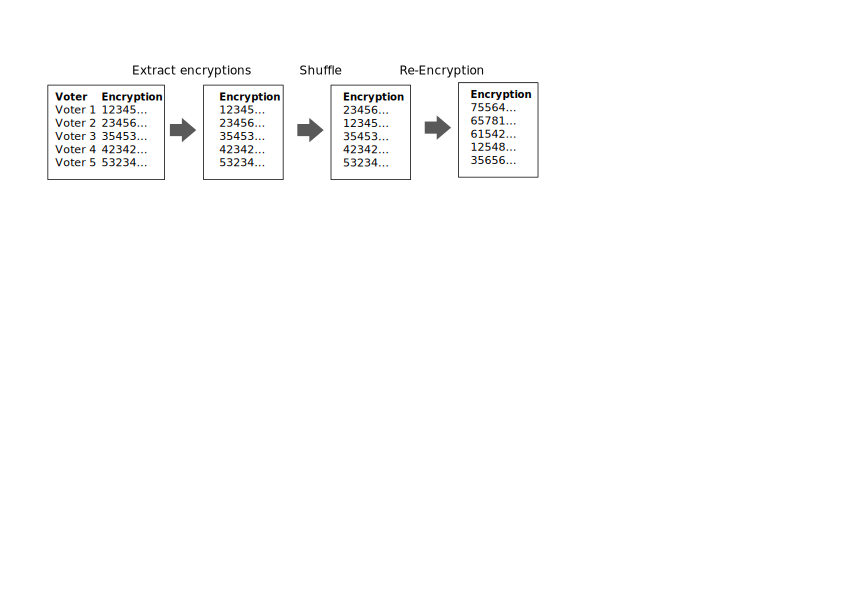
\includegraphics[scale=0.95]{assets/mixing.pdf}
\captionof{figure}{During the mixing phase, the encryptions are extracted from the list of ballots and then shuffled with a random permutation and re-encrypted by all election authorities. This measure ensures the anonymity of the votes. }\label{During the mixing}%
\end{center}

While the extraction only needs to done by the first election authority, every election authority is sequentially performing the shuffle and re-encryption on the mixed list of the previous election authority.

To prevent election authorities from cheating and not performing the mixing as specified, a proof (according to Wikström’s shuffle proof) is calculated which will be verified by all election authorities before decryption. If one of these \textbf{shuffle-proofs} fails, the election process can not proceed.

\chapter{Application Description}
In this chapter we describe the product of our bachelor thesis and the main component of our application - the visualizer web-application (front-end). We will focus mainly on the non-technical concepts as the next chapter will cover the technical aspects.

\section{Application Overview}
In an essence, all the functionality of our application revolves around visualizing an election event according to the CHVote protocol and guiding the users through the several phases. A typical CHVote election event can be broken down into phases shown in figure \ref{Phases of an election-event}

\begin{figure}
\begin{center}
\includegraphics[scale=0.65]{assets/electionStatediagram.pdf}
\captionof{figure}{In our application, an election event consists of 7 different phases (green). During the election phase, a voter can be in 3 different phases (blue)}\label{Phases of an election-event}%
\end{center}
\end{figure}

To allow the users of our application to experience and get insights about the workings of the protocol, we wanted to allow them to take the perspective of every actor of the protocol at any given time and during every phase of the election event. This is why we have divided our application into separate \textbf{views}, one for every actor:

Every actor involved in a CHVote election event has its own set of data to be displayed and specific tasks and use cases it has to perform. Most use cases are only available during a particular phase.

\begin{itemize}
	\item \textbf{Election Overview}: The election overview shows in what phase the chosen election event is currently in. Additionally, a graphical schema shows how all the actors are connected and who is involved in the current phase.
\begin{figure}
\begin{center}
\includegraphics[scale=0.50]{assets/screenshots/overview.PNG}
\captionof{figure}{The election overview guides the user through the several phases of an election event and indicates what phases have been finished and what the next steps are.}\label{Election Overview}%
\end{center}
\end{figure}

	\item \textbf{Election Administrator View}: The view of the election administrator allows a user to set-up an election event, by configuring the number of voters, the elections including the candidates and the number of selections per election. Instead of providing these information every time an election event is set up, previously defined election presets can be applied or the parameters can be generated randomly.

The election administrator view is also the place where the elections can be tallied and the final result is determined during the post-election phase.
	\item \textbf{Printing Authority View}: In the printing authority view, the voting cards can be printed and displayed for every voter. Additionally, the voting cards can be sent to the voters.

	\item \textbf{Election Authority View}: The election authority view first lets a user choose one of the three election authorities he wants to observe. On the top, new tasks will pop up whenever an election authority needs to perform a specific task such as ballot- or confirmation checking or mixing and decryption.

Additionally, the view shows the data that an election authority knows. This concept of diving a view into tasks and data, can be seen in figure \ref{Election Authority View} and has been used throughout the application and in almost every view.

\begin{figure}[p]
\begin{center}
\includegraphics[scale=0.43]{assets/screenshots/view.png}
\captionof{figure}{The election authority view as an example of how we generally structure our pages: Most views are divided into a tasks part, which allows to perform the tasks of an actor, and a data part which shows what information about an election event the participant is in possession of. }\label{Election Authority View}%
\end{center}
\end{figure}

	\item \textbf{Voter View}
	In the voter view, the vote casting process can be done for every voter that has been previously generated. The view displays both a voting form on the left, and the voters voting card on the right side. The two sensitive codes are hidden behind a scratchcard and can be copied to the voting card input by clicking on them after they have been revealed.

	\item \textbf{Bulletin Board View} The bulletin board view always shows all the data that has been appended to the bulletin board by the other actors, such as the pre-election data, the ballots that the voters have casted, as well as all the proofs generated during the post-election phase.

	\item \textbf{Verifier View}: The view of the verifier becomes visible after the election result has been published to the bulletin board and the election event has reached its final stage. By clicking on the verify button, several checks can be executed and the result is display on the page.
\end{itemize}

All the views are accessible from a tab view displayed on the top of the page which serves as our standard mean for navigation, see figure \ref{Navigation}.

\begin{figure}[p]
\begin{center}
\includegraphics[scale=0.44]{assets/screenshots/navigation.png}
\captionof{figure}{The tab beyond the page header is the main control for navigating through the different pages. It also indicates where some interaction is required next by displaying an exclamation-mark icon in the respective actors tab.}\label{Navigation}%
\end{center}
\end{figure}

From the use-cases, we tried to figure out all commonalities between the views: The views typically display the information known by the respective actor. Especially the bulletin board and election authorities will contain lots of information to be displayed. Most of the views have distinct tasks to be executed by the respective actor, such as casting a ballot in the voters view or confirming ballots from an election authorities view.

The content that a view displays, or in other words, the functionality an actor has access to, depend on the phase the election event is currently in: During the pre-election phase, the vote administrator needs to be able to set up the election while in the tallying phase, he must be able to tally and determine the final result.


\section{Design}
Given the rather large amount of complex data to be displayed, the main challenge of the project has been a well designed user interface that allows to display all important information while maintaining a clear overview.

To achieve this goal we tried to keep our design very minimalistic and follow the Google material design guidelines as much as possible by choosing an appropriate UI component framework. Even though mobile compatibility has not been a requirement, it was nevertheless our goal to make the layout as responsive as possible such that it can at least be used from a mobile phone, even though it is clearly optimized for desktop resolution.

Throughout our application we tried to establish common concepts regarding the look and feel and on how to display our data. One popular layout-concept of the Google material guidelines is the card layout. Cards can be easily integrated in a responsive grid system, look modern and allow to visually group data. In addition, we used pushover menus, tool-tips and pop-ups as they made it possible to hide lesser relevant information by default and display it only on demand of the user.

Before we started implementing our application, we have created mock-ups for most of the views, to discuss our ideas with our supervisors and incorporated their feedback as well. The following screenshots are an extract of the mock-ups in which we tried to visualize how we imagined the resulting application to look like during the conceptual phase.

% Todo: Beispiel-Bild der Mockups %

Our conceptual work also involved the development of a small prototype / proof of concept, in which we have implemented one use case in a reduced extent with the envisaged frameworks and technologies to evaluate the technical feasibility. For more information about the languages and frameworks we have decided on, we refer to the next chapter.

\chapter{Implementation Details}
In this chapter, we will describe the details on how we implemented the application. We will start explaining the architecture from a high-level perspective with each component being a blackbox. Later sections of this chapter will then further describe the internals of each component of our system.
\section{Component Overview}
From a high-level perspective, our application consists of three components which themselves may consist of multiple sub components:
\begin{itemize}
	\item Web application
	\item Backend
	\begin{itemize}
		\item REST Service
		\item Datasync Service
		\item VoteSimulation
	\end{itemize}
	\item CHVote crypto-library
\end{itemize}
%TODO: Component diagram %

\subsection{Technologies and Frameworks}
Since the CHVote crypto-library has been already implemented in python during project II, python was also the obvious choice for the backend. \textbf{Python} offers a wide variety of frameworks for building webservices. Since we planed on building a singlepage-application for the client, we chose the lightweight micro-framework flask for building a restful webservice. \textbf{Flask} also offers support for websockets and the popular websocket framework socket.io, which we used also in our frontend. \textbf{Socket.io} simplifies the usage of websockets and offers fallback technologies such as longpolling in case websocket is not supported by the browser or the webserver. For persisting the state of an election between the stateless API/webservice calls, we use mongoDB to store the states of all parties of an election.

For our frontend (web application) we evaluated several singlepage application (SPA) frameworks. \textbf{VueJS} is a new, modern and lightweight SPA framework that in contrast to Angular has a much flatter learning curve but still offered all the functionality that we needed. The VueJS addon Vuex enabled us to establish a datastore pattern in our frontend, which makes it possible to have a copy of the backend datastore in our web application which is synchronized in real-time through socket.io.

More about how these technologies and frameworks are used and the communication between these components is described in more details in the following sections.

\section{Architecture}
The core of our application is the VoteSimulation component in our backend which implements the evoting protocol by utilizing all algorithms of the CHVote crypto-library according to the CHVote specification. The VoteSimulation component internally holds the state of a whole CHVote election and exposes functions to manipulate this state at a granularity required by our web application to implement all usecases. For example: The VotingSimulation contains a list of ballots and exposes functions to cast a new ballot, which will generate a new ballot according to the protocol, by calling the CHVote crypto-library, and adds the ballot to the ballotlist.

On top of the VoteSimulation we have implemented a REST service that acts a facade to the VoteSimulation component and makes it's functionality available as an API for our webclient. The REST service also has to initialize the VoteSimulation by loading and persisting it's state from and to the database between each API call.

Since it's a requirement that all clients of a particular election must be notified of mutations of the state, we have implemented a data sync service which allows to push the state or parts of the state of the VoteSimulation to the webclients by using the websocket protocol. This service is utilized by the REST service after every API call that could have potentially manipulated the state.

To establish a proper separation of concerns, the state of the VoteSimulation is always sent to the client via the data sync service. The REST service only returns success or error codes or information that is required in response to some particular API call, and never state objects. On the other hand, the data sync service does never manipulate the state of the VoteSimulation and is solely responsible for sending data to the client.

\begin{figure}[h!]
\begin{center}
\includegraphics[scale=0.62]{assets/architecture.pdf}
\caption{Architecture}
\end{center}
\end{figure}

From the clients point of view, the webclient contains a copy of the whole VoteSimulation state in a local datastore. This store is initially populated when the web application is initialized with an election. Whenever the state of the VoteSimulation changes, the data sync service is is called to push the new data to the web application. A local mutation handler is called inside the web application which writes the new data into the local datastore.

Since the components that the webpages of the web application are built of, are directly bound to the local datastore, all mutations automatically reflected to the user. From those pages, the REST API can be called to trigger some CHVote specific action on the backend. The resulting state change is again being pushed to all clients while the responsible client that performed the HTTPS request will additionally receive a success code, or an error message in case of an error.

\section{Backend}
The backend mainly consists of the VoteSimulation which implements the CHVote protocol by using the CHVote crypto-library. 
\subsection{VoteSimulation}
We have divided the state of a CHVote election into the following classes:
\begin{itemize}
	\item BulletinBoardState: Holds all data that is publicly available on the bulletin board (the number of candidates, the tallied result)
	\item ElectionAuthorityState: Holds all data that an election authority knows (e.g. the list of ballots, the secret key of an election authority)
	\item VoterState: Since there is no distinction made between a voter and a voting client in our application, the VoterState contains the data of both the voter (e.g. the voting card) and the data typically known to the voting client (e.g. the points returned by the oblivious transfer)
	\item PrintingAuthorityState: Holds the data known to the printing authority (e.g. the list of all voters private credentials and the voting cards)
	\item ElectionAdministratorState: Holds all data known to the election administrator 
\end{itemize}

Since our application must handle multiple elections in parallel, the state cannot be kept in RAM, but needs to be persisted between every single request. For this reason we evaluated different database systems and concepts. We decided not to use a relational database system that requires us to define a database schema as we want our state objects to be the only place where the schema is defined. This makes it easier to apply changes to the protocol in future. 

For our purpose, mongoDB seemed like a good choice. Since we do not need the ability to access and filter our data with arbitrary queries, but only need to be able to save and load a state object of a particular election, we simply store the whole state as a binary string in a mongoDB collection. The only additional attribute that is saved to the database alongside with the serialized state is the electionId which denotes which election a particular state belongs to. 

An election contains multiple VoterStates and ElectionAuthorityStates. Therefore, these two states additionally require an electionAuthorityId and a voterId.

% TODO : Grafik der MongoDB collections / Struktur %

The only common functionality between every state object, is the ability to serialize the object to a JSON string. For this reason we had to write a custom transformer which tells the JSON parser how to serialize datatypes such as mpz, bytearrays and custom classes. Luckily, python offers a way to easily serialize any custom object. By calling \begin{minted}[linenos,tabsize=2,breaklines]{python}object.__dict__\end{minted} we can convert an object into a dictionary, as long as transformer is able to serialize all properties of the object.

\subsection{Actor/Party-classes}
We described how the state classes are used to divide the data of the VoteSimulation into smaller units. Similarly, the functionality of the VoteSimulation class is separated into classes, one for every actor in the protocol.

% TODO: Diagram %

The common functionality, namely, a function for loading the corresponding state from the database and one for persisting the state to the database, are contained in an abstract base class.

\subsection{REST Service}
\subsection{Data-Sync Service}

The following sequence diagram shows how the vote casting use case is implemented within the backend.
\begin{figure}[h!]
\begin{center}
\includegraphics[scale=0.65]{assets/votecastingDiagram.pdf}\\
\caption{Vote casting sequence diagram}
\end{center}
\end{figure}

\section{Crypto-library}

\subsection{Project structure}
We decided to put every algorithm of the specification in its own file together with related unit tests. The files are structured according to the actors of the protocol, for example:

\begin{itemize}
	\item \textbf{Common}: contains common cryptopgraphic algorithms and the security parameters used by multiple algorithms
	\item \textbf{ElectionAuthority}: contains all the algorithms used by the election authority
	\item \textbf{PrintingAuthority}: contains all the algorithms used by the printing authority
	\item \textbf{VotingClient}: contains all the algorithms used by the voting client
	\item \textbf{ElectionAdministration}: contains all the algorithms used by the election administrator
	\item \textbf{Utils}: contains helper classes and miscellaneous utility functions
\end{itemize}

\subsection{Public parameters}
There exist two types of public parameters:

The \textbf{security relevant parameters}, e.g:

\begin{itemize}
	\item The order of the prime groups: $p$, $\prime{p}$, $\hat{p}$
	\item The length of the voting, confirmation, return and finalization codes
	\item The number of authorities: $s$
\end{itemize}

and \textbf{public election parameters}, e.g.:

\begin{itemize}
	\item The size of the electorate: $N_E$
	\item The number of candidates: $n$
	\item The list of candidate descriptions: $c$
\end{itemize}

The security parameters are typically used within the algorithms and remain unchanged for a longer time period, whereas the public election parameters are only used by the protocol implementations and change with every election.

The object \texttt{SecurityParams} holds all security relevant parameters and is injected as an additional function argument to all algorithms. Several different \texttt{SecurityParams} objects are created initially, which contain all the parameters according to the recommendations in the CHVote specification document ("level 0" for testing purposes and "level 1" through "level 3" for actual use of the protocol). This approach allows us to use different levels of security during development of the algorithms and protocols. For simple unit testing we used "level 0" in order to inject the security parameters recommended for testing puposes. For actual test runs of the project the security parameters from "level 2" were used.

The public election parameters on the other hand are directly passed to the algorithms by the calling party. If an algorithm needs to know certain election parameters (like the size of the electorate $N_E$), these values are typically derived from vectors that they have access to, so they do not require specific knowledge of these parameters.

\subsection{Coding style}
The following source code sample shows a typical implemation of an algorithm (in this exmaple, algorithm 7.18 according to the CHVote specification).

\begin{minted}[linenos,tabsize=2,breaklines]{python}
import unittest
import os, sys
from gmpy2 import mpz
import gmpy2

sys.path.append(os.path.dirname(os.path.dirname(os.path.abspath(__file__))))

from Utils.Utils                    import AssertMpz, AssertList, AssertClass, AssertString
from Crypto.SecurityParams          import SecurityParams, secparams_l0
from Utils.ToInteger                import ToInteger
from VotingClient.GetSelectedPrimes import GetSelectedPrimes
from VotingClient.GenQuery          import GenQuery
from VotingClient.GenBallotProof    import GenBallotProof
from UnitTestParams                 import unittestparams
from Types                          import Ballot
from Utils.StringToInteger          import StringToInteger

def GenBallot(X_bold, s, pk, secparams):
    """
    Algorithm 7.18: Generates a ballot based on the selection s and the voting code X. The
    ballot includes an OT query a and a proof pi. The algorithm also returns the random
    values used to generate the OT query. These random values are required in Alg. 7.27
    to derive the transferred messages from the OT response, which itself is generated by Alg. 7.25.

    Args:
        X_bold (str):                       Voting Code X ∈ A_X^l_X
        s (list of int):                    Selection s = (s_1, ... , s_k), 1 <= s_1 < ... < s_k
        pk (mpz):                           ElGamal key pk ∈ G_p \ {1}
        secparams (SecurityParams):         Collection of public security parameters

    Returns:
        tuple:                              alpha = (r, Ballot) = (r, (x_hat, a, b, pi))
    """

    AssertMpz(pk)
    AssertList(s)
    AssertClass(secparams, SecurityParams)

    x = mpz(StringToInteger(X_bold, secparams.A_X))
    x_hat = gmpy2.powmod(secparams.g_hat, x, secparams.p_hat)

    q_bold = GetSelectedPrimes(s, secparams)                    # q = (q_1, ... , q_k)
    m = mpz(1)

    for i in range(len(q_bold)):
        m = m * q_bold[i]

    if m >= secparams.p:
        return None

    (a_bold, r_bold) = GenQuery(q_bold, pk, secparams)
    a = mpz(1)
    r = mpz(0)

    for i in range(len(a_bold)):
        a = (a * a_bold[i]) % secparams.p
        r = (r + r_bold[i]) % secparams.q

    b = gmpy2.powmod(secparams.g,r, secparams.p)
    pi = GenBallotProof(x,m,r,x_hat,a,b,pk, secparams)
    alpha = Ballot(x_hat,a_bold,b,pi)

    return (alpha, r_bold)

class GenBallotTest(unittest.TestCase):
    def testGenBallot(self):
        selection = [1,4]       # select candidates with indices 1,4
        (ballot, r) = GenBallot(unittestparams.X, selection, unittestparams.pk, secparams_l0)
        print(ballot)
        print(r)

if __name__ == '__main__':
    unittest.main()
\end{minted}

All algorithms contain a short description, which was taken as-is from the specification document, as well as a comment (Google-style documentation string), which can be used to automatically generate code documentation. The algorithm itself is implemented as close to the specification as possible, using the same variable names and (as far as the language supports it) similar control structures:

\begin{itemize}
	\item The suffix \texttt{\_bold} for emphasized (bold) variables, e.g. \texttt{p\_bold} for \textbf{p}
	\item The suffix \texttt{\_hat} for variables with a hat, e.g. \texttt{a\_hat} for $\hat{a}$
	\item The suffix \texttt{\_prime} for variables with a prime, e.g. \texttt{a\_prime} for $a'$
	\item etc.
\end{itemize}

Each file also contains unit test relevant to the specific algorithm (if unit testing was considered useful for the particular algorithm).

The following example shows the similarities between the algorithm pseudo code and the actual implmentation in Python:

\begin{multicols}{2}
%\includegraphics[width=0.46\textwidth]{images/genballot.png}
\columnbreak
\begin{minted}[fontsize=\scriptsize]{python}
x = mpz(StringToInteger(X_bold, secparams.A_X))
x_hat = gmpy2.powmod(secparams.g_hat, x, secparams.p_hat)
q_bold = GetSelectedPrimes(s, secparams)

m = mpz(1)
for i in range(len(q_bold)):
    m = m * q_bold[i]

if m >= secparams.p:
    return None

(a_bold, r_bold) = GenQuery(q_bold, pk, secparams)
a = mpz(1)
r = mpz(0)

for i in range(len(a_bold)):
    a = (a * a_bold[i]) % secparams.p
    r = (r + r_bold[i]) % secparams.q

b = gmpy2.powmod(secparams.g,r, secparams.p)
pi = GenBallotProof(x,m,r,x_hat,a,b,pk, secparams)
alpha = Ballot(x_hat,a_bold,b,pi)

return (alpha, r_bold)
\end{minted}
\end{multicols}

\subsection{Return types}
In most cases, when an algorithm returns more than a scalar datatype, tuples are used. Tuples allow to return multiple values from a function:

\begin{minted}[linenos,tabsize=2,breaklines]{python}
def foo():
   return (1, 2)

def main():
   a, b = foo()
\end{minted}

This way a lot of the source code looked very similar to the pseudo code in the CHVote specification. For more complex data types or return values that are used more often, named tuples were used. The data type "namedtuple" is like a lightweight class and allows access to named properties.

\begin{minted}[linenos,tabsize=2,breaklines]{python}
Ballot = namedtuple("Ballot", "x_hat, a_bold, b, pi")

def main():
   Ballot b = getBallot()
   x_hat = b.x_hat
\end{minted}

By following this approach we can avoid having lots of container classes only used to pass data structures between the algorithms.

\section{Frontend}
Our frontend is a singlepage application built with Javascript, VueJS, HTML5 and CSS3. We tried to follow the design patterns and best practices proposed by the VueJS framework wherever possible.

Every site of our applications consists of at least one VueJS component which is activated when the user visits the corresponding route in the URL.
\subsection{Datastore}
The web application's datastore is divided into multiple modules, one datastore module for each corresponding state of the backend.
 
%TODO: Grafik die zeigt, wie VueX Datastores mit Backend States zusammenhängen %

\chapter{Conclusion}
The new CHVote specifications seem like a real breakthrough in e-voting. Many of the technical limitations which prevented the current systems like the one of Geneva from being used as a large scale e-voting platform, can now be solved. However, e-voting must ultimately be approved both in politics as well as by the Swiss citizens. The complexity and cryptographic nature of e-voting makes it difficult for ordinary citizens to fully understand why and how this protocol works. The missing of knowledge might even result in mistrust towards e-voting. Even though the protocol is very complicated, our application allows users to gain a better understanding of e-voting by visualizing the internals of Geneva's next generation e-voting protocol. An application like ours might not be enough to reach vast majority of the population and change their opinion about e-voting. However, the authors of the CHVote specifications intend to use our application for future presentations of their protocol, which might positively influence the attitude of their audience. 

Finally, we would like to reflect on some aspects of our bachelor thesis: especially in the beginning of the project, we have underestimated the amount of work required for working out goals and a concept for the architecture and user interface. Regular meetings with our supervisors and the agile project methodology using prototyping and mockups helped a lot to create a common understanding and a concept for our application.

With all the envisaged technologies and frameworks being relatively new and without prior knowledge and experience using them, we were unsure whether we chose the right tools and if we would succeed with our concept. However, especially Vue.js turned out to be the perfect framework for developing the front-end of the application. It allowed us to rapidly develop an intuitive user-interface. Even though the framework is relatively new and lightweight, we haven't been missing any functionalities or libraries. As for the back-end, we still believe that Python isn't the best language for implementing cryptographic protocols for the reasons we mentioned in section \ref{ssec:PythonIssues}. However, these problems did not hinder us from meeting all the requirements, including the optional can-criteria. 

Especially during the first implementation phase, we were able to follow the time schedule as planned. In the second phase, we have changed the order of some of the planned features because some features required less, and some more time than we expected.

Implementing the e-voting protocol turned out to be a very enriching experience through discovering new programming languages, building up know-how in cryptography as well as deep-diving into the technology behind the e-voting protocol. This project enabled us to get a better insight into how electronic voting could look like in a few years and even contribute a small part to its future development.
\begin{thebibliography}{999}
	\bibitem{chvote}
	"CHVote System Specification", by Rolf Haenni, Reto E. Koenig, Philipp Locher and Eric Dubuis, April 11, 2017.

	\bibitem{evotinganforderungen}
	"`Anforderungskatalog für eidgenössische Volksabstimmungen mit der elektronischen Stimmabgabe"', by Bundeskanzlei BK, June 07.2014.

	\bibitem{slowpy}
	"Why Python is Slow: Looking Under the Hood", by Jake VanderPlas, see \url{http://jakevdp.github.io/blog/2014/05/09/why-python-is-slow/}

	\bibitem{slowpy2}
	"Python speed: performance tips", from the official Python wiki, see \url{https://wiki.python.org/moin/PythonSpeed/PerformanceTips}
\end{thebibliography}

\chapter{Appendix}

\section{Use Cases}
\begin{usecase}{Create new election}
  \addrow{Primary Actor}{User}
  \addrow{Description}{The system allows to create new elections}
    \addrow{Precondition}{The system shows the available elections in a list}

    \addmulrow{Main path (M)}{
        \item User clicks on "`create election"' 
        \item System demands a name for the election 
				\item User is redirected to the election overview page
				}				
\end{usecase}

\begin{usecase}{Set-up an election event}
  \addrow{Primary Actor}{Election Administrator}
  \addrow{Description}{The election administrator can set up the election. This involves the generation of the cryptographic electorate data in the backend}
    \addrow{Precondition}{An new election has been created}
    \addrow{Postcondition}{The election has the status "`Printing"'}		
    \addmulrow{Main path (M)}{
        \item Election Administrator visits the "`Election Administrator"'-view of a new election. 
        \item The system demands the following information: 
				
				\begin{itemize}					
					\item Number of parallel elections
					\item Candidates per election
					\item Number of possible selections per election event
					\item Number of voters
					\item Counting circles of the voters
				\end{itemize}	
				\item User clicks on "`Generate"' \\
				}							
\end{usecase}

\begin{usecase}{Printing of voting cards}
  \addrow{Primary Actor}{Printing Authority}
  \addrow{Description}{The printing authority generates voting cards}
    \addrow{Precondition}{The election has the status "`Printing"'}
    \addrow{Postcondition}{The election has the status "`Delivery"'}		
    \addmulrow{Main path (M)}{
        \item The election administrator visits the "`Printing Authority"'-view of an election. 
        \item The election administrator clicks on "`Print Voting Cards"' 
				\item A list of all voters is displayed 
			  \item The election administrator can select a voter to see his voting card
				}							
\end{usecase}


\begin{usecase}{Delivery of voting cards}
  \addrow{Primary Actor}{Printing Authority}
  \addrow{Description}{The printing authority can send the voting cards to the voters}
    \addrow{Precondition}{The election has the status "`Delivery"'}
    \addrow{Postcondition}{The election has the status "`Election Phase"'}		
    \addmulrow{Main path (M)}{
        \item The election administrator visits the "`Printing Authority"'-view of an election. 
        \item The election administrator clicks on "`Deliver Voting Cards"' 
				\item Within the voters-view, the voting card shows up for every voter
				}							
\end{usecase}

\begin{usecase}{Confirmation of a vote}
  \addrow{Primary Actor}{Voter}
  \addrow{Description}{The voter can confirm his vote by verifying the verification codes and entering his confirmation code}
    \addrow{Precondition}{
		
		\begin{itemize}
			\item The election has the status "`Election Phase"'
			\item A voter is selected in the "`Voter"'-view
			\item The voter has the status "`Confirmation Phase"'
		\end{itemize}		}
    \addrow{Postcondition}{	
			The first election authority receives a "`Check-confirmation task"'	
		}		
    \addmulrow{Main path (M)}{
        \item The voter visits the "`Voter"'-view and select the corresponding voter from a list
				\item The system displays the verification codes of the selected candidates
				\item The voter must manually verify that the displayed codes match the verification codes of the selected candidates on his voting card
				\item The system demands the confirmation code
				\item The voter clicks on "`Confirm vote"'

				}							
\end{usecase}

\begin{usecase}{Checking a ballot}
  \addrow{Primary Actor}{Election Authority}
  \addrow{Description}{The election authority can verify the validity of a ballot and respond to the voters query}
    \addrow{Precondition}{
		\begin{itemize}
			\item The election has the status "`Election Phase"'
			\item The currently selected election authority has a new "`Check ballot task"'
		\end{itemize}		}
    \addrow{Postcondition}{
		
		\begin{itemize}
			\item The next election authority receives a "`Check ballot task"'
			\item If this election authority was the last one, and the ballot was valid, the voter now has the status "`Confirmation Phase"'
		\end{itemize}
		}		
    \addmulrow{Main path (M)}{
        \item The user visits the "`Election Authority"'-view and select one of the available election authorities that has new "`Check ballot task"'
				\item The system displays the query, the ballot proof and the voting credential of the voter
				\item The user click on "`Check validity"'
				\item The system displays the result of the validity check
				\item The user clicks on "`Respond"'
				}							
\end{usecase}

\begin{usecase}{Checking a confirmation}
  \addrow{Primary Actor}{Election Authority}
  \addrow{Description}{The election authority can verify the validity of a confirmation and respond to the voters query}
    \addrow{Precondition}{
		\begin{itemize}
			\item The election has the status "`Election Phase"'
			\item The currently selected election authority has a new "`Check ballot task"'
		\end{itemize}		}
    \addrow{Postcondition}{
		
		\begin{itemize}
			\item The next election authority receives a "`Check confirmation task"'
			\item If this election authority was the last one, and the confirmation was valid, the voter now has the status "`Finalization Phase"'
		\end{itemize}
		}		
    \addmulrow{Main path (M)}{
        \item The user visits the "`Election Authority"'-view and select one of the available election authorities that has new "`Check confirmation task"'
				\item The system displays information about the confirmation
				\item The user click on "`Check validity"'
				\item The system displays the result of the validity check
				\item The user clicks on "`Finalize"'
				}							
\end{usecase}

\begin{usecase}{Mixing}
  \addrow{Primary Actor}{Election Authority}
  \addrow{Description}{Every election authority can perform the mixing on the extracted list of encryptions}
    \addrow{Precondition}{
		\begin{itemize}
			\item The election has the status "`Mixing"'
			\item The previous election authority has already performed the mixing
		\end{itemize}		}
    \addrow{Postcondition}{
		
		\begin{itemize}
			\item The next election authority is able to mix
		\end{itemize}
		}		
    \addmulrow{Main path (M)}{
        \item The user visits the "`Election Authority"'-view and select one of the available election authorities that hasn't mixed before
				\item The system displays the list of encryptions of the previous election authority (or the first one in case the first election authority is selected)
				\item The user clicks on "`Mix"'
				\item The new, mixed list of encryptions is added to the known data of this election authority
				}							
\end{usecase}


\begin{usecase}{Decryption}
  \addrow{Primary Actor}{Election Authority}
  \addrow{Description}{Every election authority can perform the (partial) decryption}
    \addrow{Precondition}{
		\begin{itemize}
			\item The election has the status "`Decryption"'
			\item The previous election authority has already performed the decryption
		\end{itemize}		}
    \addrow{Postcondition}{
		\begin{itemize}
			\item The next election authority is able to decrypt
		\end{itemize}
		}		
    \addmulrow{Main path (M)}{
        \item The user visits the "`Election Authority"'-view and select one of the available election authorities that hasn't decrypted before
				\item The system displays the list of encryptions
				\item The user clicks on "`Decrypt"'
				\item The list of partial decryptions is added to the known data of this election authority
				}							
\end{usecase}


\begin{usecase}{Tallying}
  \addrow{Primary Actor}{Election Administrator}
  \addrow{Description}{The election administrator can perform the tallying and view the final result}
    \addrow{Precondition}{
		The election has the status "`Tallying"'
		}
    \addrow{Postcondition}{
		The has the status "`Finished"'
		}		
    \addmulrow{Main path (M)}{
        \item The user visits the "`Election Administrator"'-view
				\item The user clicks on "`Tally"'
				\item The final result is added to the known data of the election administrator
				}							
\end{usecase}

\section{Test-Cases}
\begin{testcase}{Pre-Election}
  \addrow{Description}{This test covers all the pre-election steps, including the creation of a new election, setting it up from the election administration view and the printing- and delivery of the voting cards}
    \addrow{Precondition}{	
		}
    \addrow{Postcondition}{	
		\begin{itemize}
			\item The election event is in the status "`Election"'
			\item The voters have received a voting card
		\end{itemize}
		}		
    \addstepsrow{Steps}{
        \item Start our application
				\item Choose \textbf{Election Events} from the main menu
				\item Click on \textbf{\textit{Create new election event}}
				\item Enter a name for the election event and choose a security level and click on \textbf{\textit{create}}
				\item The \textbf{Election Admin} tab should now have an interaction notification
				\item Visit the \textbf{Election Admin} view
				\item Enter at least 3 for the number of voters, at least 3 different candidates and 1 for the number of selection and click on \textbf{\textit{Setup Election Event}} 
				\item The \textbf{Printing Authority} tab should now have an interaction notification
				\item Visit the \textbf{Printing Authority} view
				\item Click on \textbf{Print Voting Cards}
				\item The voting cards for all voters should now be displayed
				\item Click on \textbf{Deliver Voting Cards To Voters}
				\item The voting cards should now disappear and the \textbf{Voters} tab should now have an interaction notification
				\item Visit the Voters view, select a voter and check that the voting card is displayed correctly
				}							
\end{testcase}

\begin{testcase}{Election}
  \addrow{Test-Case}{2. Election}
  \addrow{Description}{This test covers the election phase in which a voter casts and confirms a ballot and the election authorities checks the ballots and confirmations and responds to the voter.}
    \addrow{Precondition}{
		\begin{itemize}
			\item The election event has been set up appropriately as described in test-case 1.
			\item The second and third election authorities should have automatic task processing enabled
		\end{itemize}		}
    \addrow{Postcondition}{
		
		\begin{itemize}
			\item The election event is in the status "`Election"'
			\item There are at least 3 confirmed ballots
		\end{itemize}
		}		
    \addstepsrow{Steps}{     
				\item Visit the \textbf{Voters} view and select voter 1
				\item Check the box for candidate 1 in the vote casting form
				\item Scratch open the voting code on your voting card and click on the revealed code. The code should be copied into the \textbf{voting code} input field
				\item Click on \textbf{Cast vote}			
				\item Visit the \textbf{Election Authority} view and click on the first election authority
				\item There should be a check-ballot task for voter 1. Click on \textbf{Check Validity} to check the ballot. The ballot should be valid. Click on \textbf{Respond}. 
				\item The ballot should be added to the ballot list of this election authority. Verify that the ballot is also contained in the bulletin boards ballot list!
				\item Return to the voters view. The voter should be prompted to verify that the returned verification codes match. If so, reveal your confirmation code and click it to copy it to the input field. Click on "`Confirm Vote"'
				\item Visit the \textbf{Election Authority} view and click on the first election authority
				\item There should be a check-confirmation task for voter 1. Click on \textbf{Check Validity} to check the confirmation. The confirmation should be valid. Click on \textbf{Finalize}. 
				\item The ballot list should now display the ballot as "`confirmed"'. The confirmation should also show up in the confirmation list if you expand the ballot.
				\item Return to the voters view. The voter should now see the returned finalization code that should match the code on the voting card
				\item Repeat this test-case for voter 2 and voter 3, choosing the second candidate for voter 2 and the third candidate for voter 3
				}							
\end{testcase}

\begin{testcase}{Post-Election}
  \addrow{Test-Case}{3. Post-Election}
  \addrow{Description}{This test covers the post-election phases: mixing, decryption, tallying and verification}
    \addrow{Precondition}{
		\begin{itemize}
			\item The election event has been set up appropriately as described in test-case 1.
			\item 3 voters have casted their vote according to test-case 2.
		\end{itemize}		}
    \addrow{Postcondition}{	
		\begin{itemize}
			\item The election event is in the status "`Finished"'
			\item The verification has succeed and the correct election result is published on the bulletin board
		\end{itemize}
		}		
    \addstepsrow{Steps}{     
				\item Visit the \textbf{Election Administrator} view
				\item Click on \textbf{End Election Phase and Start Mixing}
				\item Visit the \textbf{Election Authority} view and choose the election authority 1
				\item Click on \textbf{Mix}			
				\item You should see the list of encryptions being shuffled and re-encrypted. The result should be added to the data. The same should automatically have happened for the other election authorities.
				\item Visit the \textbf{Election Administrator} view and click on \textbf{Start Decryption}
				\item Visit the \textbf{Election Authority} view and choose the election authority 1
				\item Click on \textbf{Decrypt}	
				\item The partially decrypted data should appear in the election authority data. The same should have happened for the other election authorities.
				\item Visit the \textbf{Election Administrator} view and click on \textbf{Tally}
				\item Under data, you should see the decrypted votes and the final result in a text- and chart representation.
				\item Click on \textbf{Publish Result} and visit the \textbf{Bulletin Board} view
				\item The bulletin board should now also contain show the result of the election event.
				\item Visit the \textbf{Verifier} view and click on \textbf{Verify Election}
				\item All checks should show a green icon and succeed.
				}							
\end{testcase}






\end{document}
